\documentclass[1p]{elsarticle_modified}
%\bibliographystyle{elsarticle-num}

%\usepackage[colorlinks]{hyperref}
%\usepackage{abbrmath_seonhwa} %\Abb, \Ascr, \Acal ,\Abf, \Afrak
\usepackage{amsfonts}
\usepackage{amssymb}
\usepackage{amsmath}
\usepackage{amsthm}
\usepackage{scalefnt}
\usepackage{amsbsy}
\usepackage{kotex}
\usepackage{caption}
\usepackage{subfig}
\usepackage{color}
\usepackage{graphicx}
\usepackage{xcolor} %% white, black, red, green, blue, cyan, magenta, yellow
\usepackage{float}
\usepackage{setspace}
\usepackage{hyperref}

\usepackage{tikz}
\usetikzlibrary{arrows}

\usepackage{multirow}
\usepackage{array} % fixed length table
\usepackage{hhline}

%%%%%%%%%%%%%%%%%%%%%
\makeatletter
\renewcommand*\env@matrix[1][\arraystretch]{%
	\edef\arraystretch{#1}%
	\hskip -\arraycolsep
	\let\@ifnextchar\new@ifnextchar
	\array{*\c@MaxMatrixCols c}}
\makeatother %https://tex.stackexchange.com/questions/14071/how-can-i-increase-the-line-spacing-in-a-matrix
%%%%%%%%%%%%%%%

\usepackage[normalem]{ulem}

\newcommand{\msout}[1]{\ifmmode\text{\sout{\ensuremath{#1}}}\else\sout{#1}\fi}
%SOURCE: \msout is \stkout macro in https://tex.stackexchange.com/questions/20609/strikeout-in-math-mode

\newcommand{\cancel}[1]{
	\ifmmode
	{\color{red}\msout{#1}}
	\else
	{\color{red}\sout{#1}}
	\fi
}

\newcommand{\add}[1]{
	{\color{blue}\uwave{#1}}
}

\newcommand{\replace}[2]{
	\ifmmode
	{\color{red}\msout{#1}}{\color{blue}\uwave{#2}}
	\else
	{\color{red}\sout{#1}}{\color{blue}\uwave{#2}}
	\fi
}

\newcommand{\Sol}{\mathcal{S}} %segment
\newcommand{\D}{D} %diagram
\newcommand{\A}{\mathcal{A}} %arc


%%%%%%%%%%%%%%%%%%%%%%%%%%%%%5 test

\def\sl{\operatorname{\textup{SL}}(2,\Cbb)}
\def\psl{\operatorname{\textup{PSL}}(2,\Cbb)}
\def\quan{\mkern 1mu \triangleright \mkern 1mu}

\theoremstyle{definition}
\newtheorem{thm}{Theorem}[section]
\newtheorem{prop}[thm]{Proposition}
\newtheorem{lem}[thm]{Lemma}
\newtheorem{ques}[thm]{Question}
\newtheorem{cor}[thm]{Corollary}
\newtheorem{defn}[thm]{Definition}
\newtheorem{exam}[thm]{Example}
\newtheorem{rmk}[thm]{Remark}
\newtheorem{alg}[thm]{Algorithm}

\newcommand{\I}{\sqrt{-1}}
\begin{document}

%\begin{frontmatter}
%
%\title{Boundary parabolic representations of knots up to 8 crossings}
%
%%% Group authors per affiliation:
%\author{Yunhi Cho} 
%\address{Department of Mathematics, University of Seoul, Seoul, Korea}
%\ead{yhcho@uos.ac.kr}
%
%
%\author{Seonhwa Kim} %\fnref{s_kim}}
%\address{Center for Geometry and Physics, Institute for Basic Science, Pohang, 37673, Korea}
%\ead{ryeona17@ibs.re.kr}
%
%\author{Hyuk Kim}
%\address{Department of Mathematical Sciences, Seoul National University, Seoul 08826, Korea}
%\ead{hyukkim@snu.ac.kr}
%
%\author{Seokbeom Yoon}
%\address{Department of Mathematical Sciences, Seoul National University, Seoul, 08826,  Korea}
%\ead{sbyoon15@snu.ac.kr}
%
%\begin{abstract}
%We find all boundary parabolic representation of knots up to 8 crossings.
%
%\end{abstract}
%\begin{keyword}
%    \MSC[2010] 57M25 
%\end{keyword}
%
%\end{frontmatter}

%\linenumbers
%\tableofcontents
%
\newcommand\colored[1]{\textcolor{white}{\rule[-0.35ex]{0.8em}{1.4ex}}\kern-0.8em\color{red} #1}%
%\newcommand\colored[1]{\textcolor{white}{ #1}\kern-2.17ex	\textcolor{white}{ #1}\kern-1.81ex	\textcolor{white}{ #1}\kern-2.15ex\color{red}#1	}

{\Large $\underline{12a_{0806}~(K12a_{0806})}$}

\setlength{\tabcolsep}{10pt}
\renewcommand{\arraystretch}{1.6}
\vspace{1cm}\begin{tabular}{m{100pt}>{\centering\arraybackslash}m{274pt}}
\multirow{5}{120pt}{
	\centering
	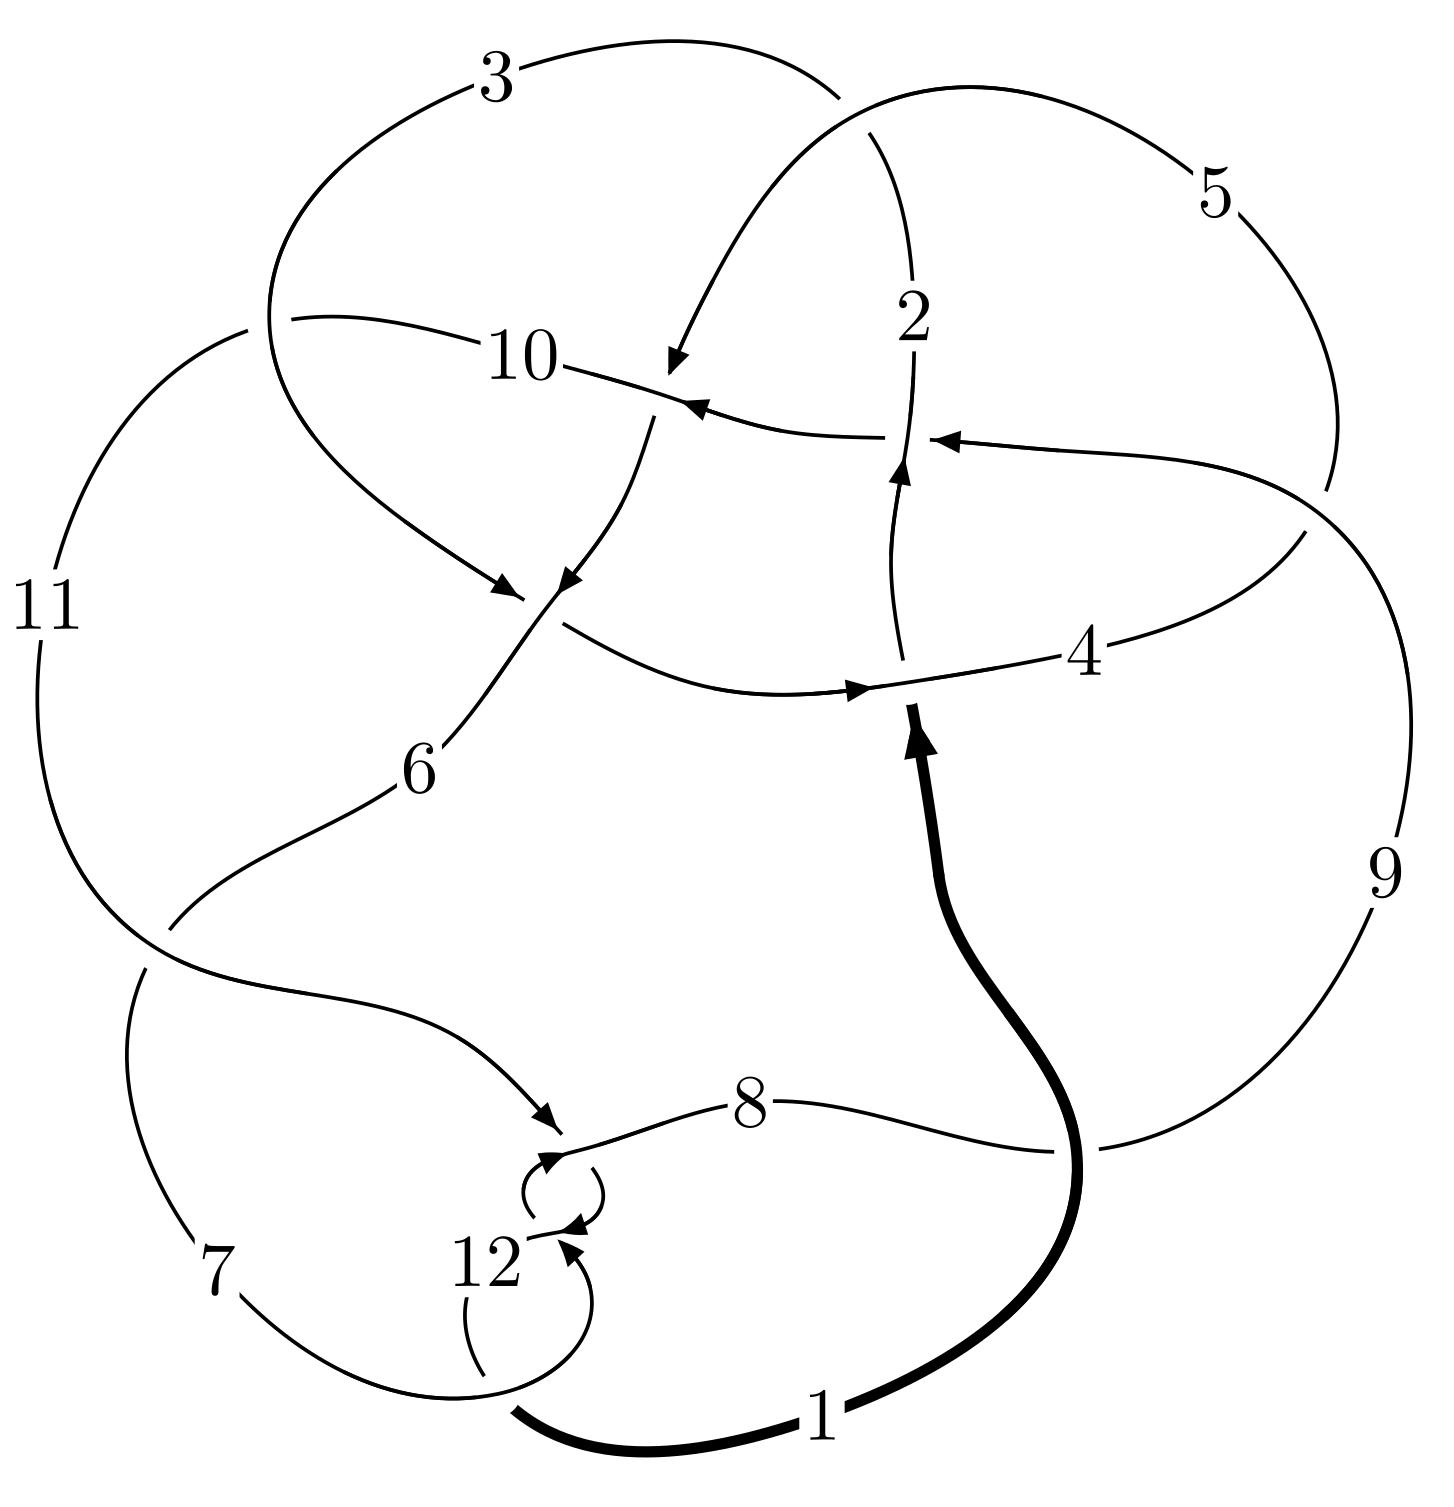
\includegraphics[width=112pt]{../../../GIT/diagram.site/Diagrams/png/1607_12a_0806.png}\\
\ \ \ A knot diagram\footnotemark}&
\allowdisplaybreaks
\textbf{Linearized knot diagam} \\
\cline{2-2}
 &
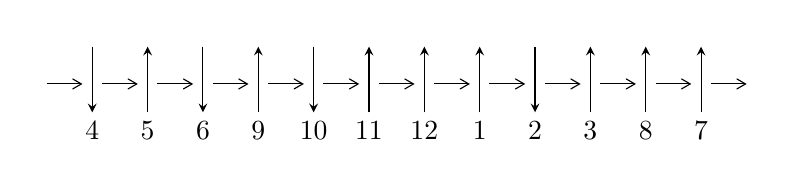
\begin{tikzpicture}[x=20pt, y=17pt]
	% nodes
	\node (C0) at (0, 0) {};
	\node (C1) at (1, 0) {};
	\node (C1U) at (1, +1) {};
	\node (C1D) at (1, -1) {4};

	\node (C2) at (2, 0) {};
	\node (C2U) at (2, +1) {};
	\node (C2D) at (2, -1) {5};

	\node (C3) at (3, 0) {};
	\node (C3U) at (3, +1) {};
	\node (C3D) at (3, -1) {6};

	\node (C4) at (4, 0) {};
	\node (C4U) at (4, +1) {};
	\node (C4D) at (4, -1) {9};

	\node (C5) at (5, 0) {};
	\node (C5U) at (5, +1) {};
	\node (C5D) at (5, -1) {10};

	\node (C6) at (6, 0) {};
	\node (C6U) at (6, +1) {};
	\node (C6D) at (6, -1) {11};

	\node (C7) at (7, 0) {};
	\node (C7U) at (7, +1) {};
	\node (C7D) at (7, -1) {12};

	\node (C8) at (8, 0) {};
	\node (C8U) at (8, +1) {};
	\node (C8D) at (8, -1) {1};

	\node (C9) at (9, 0) {};
	\node (C9U) at (9, +1) {};
	\node (C9D) at (9, -1) {2};

	\node (C10) at (10, 0) {};
	\node (C10U) at (10, +1) {};
	\node (C10D) at (10, -1) {3};

	\node (C11) at (11, 0) {};
	\node (C11U) at (11, +1) {};
	\node (C11D) at (11, -1) {8};

	\node (C12) at (12, 0) {};
	\node (C12U) at (12, +1) {};
	\node (C12D) at (12, -1) {7};
	\node (C13) at (13, 0) {};

	% arrows
	\draw[->,>={angle 60}]
	(C0) edge (C1) (C1) edge (C2) (C2) edge (C3) (C3) edge (C4) (C4) edge (C5) (C5) edge (C6) (C6) edge (C7) (C7) edge (C8) (C8) edge (C9) (C9) edge (C10) (C10) edge (C11) (C11) edge (C12) (C12) edge (C13) ;	\draw[->,>=stealth]
	(C1U) edge (C1D) (C2D) edge (C2U) (C3U) edge (C3D) (C4D) edge (C4U) (C5U) edge (C5D) (C6D) edge (C6U) (C7D) edge (C7U) (C8D) edge (C8U) (C9U) edge (C9D) (C10D) edge (C10U) (C11D) edge (C11U) (C12D) edge (C12U) ;
	\end{tikzpicture} \\
\hhline{~~} \\& 
\textbf{Solving Sequence} \\ \cline{2-2} 
 &
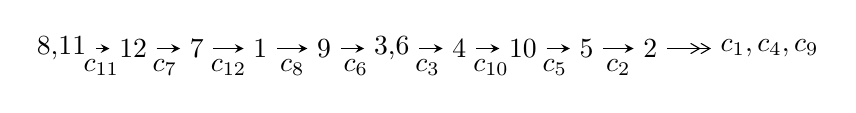
\begin{tikzpicture}[x=23pt, y=7pt]
	% node
	\node (A0) at (-1/8, 0) {8,11};
	\node (A1) at (1, 0) {12};
	\node (A2) at (2, 0) {7};
	\node (A3) at (3, 0) {1};
	\node (A4) at (4, 0) {9};
	\node (A5) at (81/16, 0) {3,6};
	\node (A6) at (49/8, 0) {4};
	\node (A7) at (57/8, 0) {10};
	\node (A8) at (65/8, 0) {5};
	\node (A9) at (73/8, 0) {2};
	\node (C1) at (1/2, -1) {$c_{11}$};
	\node (C2) at (3/2, -1) {$c_{7}$};
	\node (C3) at (5/2, -1) {$c_{12}$};
	\node (C4) at (7/2, -1) {$c_{8}$};
	\node (C5) at (9/2, -1) {$c_{6}$};
	\node (C6) at (45/8, -1) {$c_{3}$};
	\node (C7) at (53/8, -1) {$c_{10}$};
	\node (C8) at (61/8, -1) {$c_{5}$};
	\node (C9) at (69/8, -1) {$c_{2}$};
	\node (A10) at (11, 0) {$c_{1},c_{4},c_{9}$};

	% edge
	\draw[->,>=stealth]	
	(A0) edge (A1) (A1) edge (A2) (A2) edge (A3) (A3) edge (A4) (A4) edge (A5) (A5) edge (A6) (A6) edge (A7) (A7) edge (A8) (A8) edge (A9) ;
	\draw[->>,>={angle 60}]	
	(A9) edge (A10);
\end{tikzpicture} \\ 

\end{tabular} \\

\footnotetext{
The image of knot diagram is generated by the software ``\textbf{Draw programme}" developed by Andrew Bartholomew(\url{http://www.layer8.co.uk/maths/draw/index.htm\#Running-draw}), where we modified some parts for our purpose(\url{https://github.com/CATsTAILs/LinksPainter}).
}\phantom \\ \newline 
\centering \textbf{Ideals for irreducible components\footnotemark of $X_{\text{par}}$} 
 
\begin{align*}
I^u_{1}&=\langle 
17065 u^{50}+58132 u^{49}+\cdots+10949 b+696131,\\
\phantom{I^u_{1}}&\phantom{= \langle  }-681303 u^{50}-3569366 u^{49}+\cdots+120439 a-14235505,\;u^{51}+6 u^{50}+\cdots+17 u+11\rangle \\
I^u_{2}&=\langle 
768 u^{38} a+2716 u^{38}+\cdots-4526 a-10377,\;-5 u^{38} a+5 u^{38}+\cdots-10 a+2,\;u^{39}-2 u^{38}+\cdots+4 u-1\rangle \\
I^u_{3}&=\langle 
- u^{10}-4 u^8-5 u^6+u^3+4 u^2+b+2 u+1,\\
\phantom{I^u_{3}}&\phantom{= \langle  }u^{12}+u^{11}+5 u^{10}+4 u^9+9 u^8+5 u^7+4 u^6- u^5-7 u^4-7 u^3-7 u^2+a-3 u+1,\\
\phantom{I^u_{3}}&\phantom{= \langle  }u^{15}+u^{14}+7 u^{13}+6 u^{12}+19 u^{11}+14 u^{10}+22 u^9+13 u^8+u^7-4 u^6-22 u^5-17 u^4-16 u^3-10 u^2- u-1\rangle \\
I^u_{4}&=\langle 
a u- u^2+b+u-1,\;-3 u^2 a+a^2-3 a- u+1,\;u^3- u^2+2 u-1\rangle \\
\\
I^v_{1}&=\langle 
a,\;b-1,\;v+1\rangle \\
\end{align*}
\raggedright * 5 irreducible components of $\dim_{\mathbb{C}}=0$, with total 151 representations.\\
\footnotetext{All coefficients of polynomials are rational numbers. But the coefficients are sometimes approximated in decimal forms when there is not enough margin.}
\newpage
\renewcommand{\arraystretch}{1}
\centering \section*{I. $I^u_{1}= \langle 17065 u^{50}+58132 u^{49}+\cdots+10949 b+696131,\;-6.81\times10^{5} u^{50}-3.57\times10^{6} u^{49}+\cdots+1.20\times10^{5} a-1.42\times10^{7},\;u^{51}+6 u^{50}+\cdots+17 u+11 \rangle$}
\flushleft \textbf{(i) Arc colorings}\\
\begin{tabular}{m{7pt} m{180pt} m{7pt} m{180pt} }
\flushright $a_{8}=$&$\begin{pmatrix}0\\u\end{pmatrix}$ \\
\flushright $a_{11}=$&$\begin{pmatrix}1\\0\end{pmatrix}$ \\
\flushright $a_{12}=$&$\begin{pmatrix}1\\- u^2\end{pmatrix}$ \\
\flushright $a_{7}=$&$\begin{pmatrix}- u\\u^3+u\end{pmatrix}$ \\
\flushright $a_{1}=$&$\begin{pmatrix}u^2+1\\- u^4-2 u^2\end{pmatrix}$ \\
\flushright $a_{9}=$&$\begin{pmatrix}u^5+2 u^3+u\\- u^7-3 u^5-2 u^3+u\end{pmatrix}$ \\
\flushright $a_{3}=$&$\begin{pmatrix}5.65683 u^{50}+29.6363 u^{49}+\cdots+12.5028 u+118.197\\-1.55859 u^{50}-5.30934 u^{49}+\cdots+30.0563 u-63.5794\end{pmatrix}$ \\
\flushright $a_{6}=$&$\begin{pmatrix}- u^3-2 u\\u^3+u\end{pmatrix}$ \\
\flushright $a_{4}=$&$\begin{pmatrix}8.37881 u^{50}+48.7374 u^{49}+\cdots+50.8618 u+144.760\\-1.53548 u^{50}-10.7228 u^{49}+\cdots+2.32012 u-92.1670\end{pmatrix}$ \\
\flushright $a_{10}=$&$\begin{pmatrix}-6.19247 u^{50}-28.1472 u^{49}+\cdots+13.9193 u-64.2872\\10.0141 u^{50}+55.3135 u^{49}+\cdots+59.6389 u+98.3815\end{pmatrix}$ \\
\flushright $a_{5}=$&$\begin{pmatrix}3.63966 u^{50}+23.9159 u^{49}+\cdots+51.3463 u+6.74407\\-0.613389 u^{50}-7.84263 u^{49}+\cdots-28.5497 u-51.1307\end{pmatrix}$ \\
\flushright $a_{2}=$&$\begin{pmatrix}4.64825 u^{50}+26.2761 u^{49}+\cdots+23.4246 u+101.470\\-1.61339 u^{50}-6.84263 u^{49}+\cdots+21.4503 u-51.1307\end{pmatrix}$\\&\end{tabular}
\flushleft \textbf{(ii) Obstruction class $= -1$}\\~\\
\flushleft \textbf{(iii) Cusp Shapes $= \frac{138745}{10949} u^{50}+\frac{762715}{10949} u^{49}+\cdots+\frac{578532}{10949} u+\frac{1808552}{10949}$}\\~\\
\newpage\renewcommand{\arraystretch}{1}
\flushleft \textbf{(iv) u-Polynomials at the component}\newline \\
\begin{tabular}{m{50pt}|m{274pt}}
Crossings & \hspace{64pt}u-Polynomials at each crossing \\
\hline $$\begin{aligned}c_{1},c_{3}\end{aligned}$$&$\begin{aligned}
&u^{51}+8 u^{50}+\cdots- u+1
\end{aligned}$\\
\hline $$\begin{aligned}c_{2}\end{aligned}$$&$\begin{aligned}
&u^{51}+27 u^{50}+\cdots-21 u-11
\end{aligned}$\\
\hline $$\begin{aligned}c_{4},c_{10}\end{aligned}$$&$\begin{aligned}
&u^{51}-8 u^{49}+\cdots-7 u+3
\end{aligned}$\\
\hline $$\begin{aligned}c_{5},c_{9}\end{aligned}$$&$\begin{aligned}
&u^{51}-17 u^{49}+\cdots-3 u+1
\end{aligned}$\\
\hline $$\begin{aligned}c_{6},c_{8}\end{aligned}$$&$\begin{aligned}
&u^{51}+6 u^{50}+\cdots-13127 u-1727
\end{aligned}$\\
\hline $$\begin{aligned}c_{7},c_{11},c_{12}\end{aligned}$$&$\begin{aligned}
&u^{51}-6 u^{50}+\cdots+17 u-11
\end{aligned}$\\
\hline
\end{tabular}\\~\\
\newpage\renewcommand{\arraystretch}{1}
\flushleft \textbf{(v) Riley Polynomials at the component}\newline \\
\begin{tabular}{m{50pt}|m{274pt}}
Crossings & \hspace{64pt}Riley Polynomials at each crossing \\
\hline $$\begin{aligned}c_{1},c_{3}\end{aligned}$$&$\begin{aligned}
&y^{51}-12 y^{50}+\cdots+41 y-1
\end{aligned}$\\
\hline $$\begin{aligned}c_{2}\end{aligned}$$&$\begin{aligned}
&y^{51}- y^{50}+\cdots+265 y-121
\end{aligned}$\\
\hline $$\begin{aligned}c_{4},c_{10}\end{aligned}$$&$\begin{aligned}
&y^{51}-16 y^{50}+\cdots+109 y-9
\end{aligned}$\\
\hline $$\begin{aligned}c_{5},c_{9}\end{aligned}$$&$\begin{aligned}
&y^{51}-34 y^{50}+\cdots+63 y-1
\end{aligned}$\\
\hline $$\begin{aligned}c_{6},c_{8}\end{aligned}$$&$\begin{aligned}
&y^{51}-46 y^{50}+\cdots+6018391 y-2982529
\end{aligned}$\\
\hline $$\begin{aligned}c_{7},c_{11},c_{12}\end{aligned}$$&$\begin{aligned}
&y^{51}+42 y^{50}+\cdots+751 y-121
\end{aligned}$\\
\hline
\end{tabular}\\~\\
\newpage\flushleft \textbf{(vi) Complex Volumes and Cusp Shapes}
$$\begin{array}{c|c|c}  
\text{Solutions to }I^u_{1}& \I (\text{vol} + \sqrt{-1}CS) & \text{Cusp shape}\\
 \hline 
\begin{aligned}
u &= -0.957849 + 0.091145 I \\
a &= -1.008770 - 0.320069 I \\
b &= \phantom{-}0.552197 + 0.030702 I\end{aligned}
 & \phantom{-}5.37004 - 0.21205 I & \phantom{-}11.7933 + 19.3332 I \\ \hline\begin{aligned}
u &= -0.957849 - 0.091145 I \\
a &= -1.008770 + 0.320069 I \\
b &= \phantom{-}0.552197 - 0.030702 I\end{aligned}
 & \phantom{-}5.37004 + 0.21205 I & \phantom{-}11.7933 - 19.3332 I \\ \hline\begin{aligned}
u &= -0.872610 + 0.107152 I \\
a &= \phantom{-}2.73299 - 0.35546 I \\
b &= -1.35191 + 0.89094 I\end{aligned}
 & \phantom{-}6.3580 - 14.4453 I & \phantom{-}7.77501 + 8.25655 I \\ \hline\begin{aligned}
u &= -0.872610 - 0.107152 I \\
a &= \phantom{-}2.73299 + 0.35546 I \\
b &= -1.35191 - 0.89094 I\end{aligned}
 & \phantom{-}6.3580 + 14.4453 I & \phantom{-}7.77501 - 8.25655 I \\ \hline\begin{aligned}
u &= \phantom{-}0.850284\phantom{ +0.000000I} \\
a &= -2.37050\phantom{ +0.000000I} \\
b &= \phantom{-}1.10715\phantom{ +0.000000I}\end{aligned}
 & \phantom{-}7.35958\phantom{ +0.000000I} & \phantom{-}12.9810\phantom{ +0.000000I} \\ \hline\begin{aligned}
u &= -0.841318 + 0.059912 I \\
a &= -1.61858 + 0.39625 I \\
b &= \phantom{-}0.651279 - 0.942262 I\end{aligned}
 & \phantom{-}3.92874 - 5.39698 I & \phantom{-}1.33611 + 5.91219 I \\ \hline\begin{aligned}
u &= -0.841318 - 0.059912 I \\
a &= -1.61858 - 0.39625 I \\
b &= \phantom{-}0.651279 + 0.942262 I\end{aligned}
 & \phantom{-}3.92874 + 5.39698 I & \phantom{-}1.33611 - 5.91219 I \\ \hline\begin{aligned}
u &= -0.110159 + 1.171870 I \\
a &= -0.653100 - 0.676264 I \\
b &= \phantom{-}0.747128 - 0.387182 I\end{aligned}
 & -2.43106 - 2.02323 I & \phantom{-0.000000 } 0 \\ \hline\begin{aligned}
u &= -0.110159 - 1.171870 I \\
a &= -0.653100 + 0.676264 I \\
b &= \phantom{-}0.747128 + 0.387182 I\end{aligned}
 & -2.43106 + 2.02323 I & \phantom{-0.000000 } 0 \\ \hline\begin{aligned}
u &= \phantom{-}0.793654\phantom{ +0.000000I} \\
a &= \phantom{-}3.77720\phantom{ +0.000000I} \\
b &= -1.59505\phantom{ +0.000000I}\end{aligned}
 & \phantom{-}2.43906\phantom{ +0.000000I} & \phantom{-}4.56150\phantom{ +0.000000I}\\
 \hline 
 \end{array}$$\newpage$$\begin{array}{c|c|c}  
\text{Solutions to }I^u_{1}& \I (\text{vol} + \sqrt{-1}CS) & \text{Cusp shape}\\
 \hline 
\begin{aligned}
u &= \phantom{-}0.536539 + 0.581907 I \\
a &= \phantom{-}0.286173 - 1.079810 I \\
b &= -0.871692 + 0.727547 I\end{aligned}
 & -0.20392 - 5.98050 I & \phantom{-}4.39957 + 5.96035 I \\ \hline\begin{aligned}
u &= \phantom{-}0.536539 - 0.581907 I \\
a &= \phantom{-}0.286173 + 1.079810 I \\
b &= -0.871692 - 0.727547 I\end{aligned}
 & -0.20392 + 5.98050 I & \phantom{-}4.39957 - 5.96035 I \\ \hline\begin{aligned}
u &= -0.437498 + 1.162750 I \\
a &= -0.949926 - 0.859681 I \\
b &= \phantom{-}1.31754 + 0.83680 I\end{aligned}
 & \phantom{-}3.12029 + 9.75993 I & \phantom{-0.000000 } 0 \\ \hline\begin{aligned}
u &= -0.437498 - 1.162750 I \\
a &= -0.949926 + 0.859681 I \\
b &= \phantom{-}1.31754 - 0.83680 I\end{aligned}
 & \phantom{-}3.12029 - 9.75993 I & \phantom{-0.000000 } 0 \\ \hline\begin{aligned}
u &= -0.526323 + 1.137400 I \\
a &= \phantom{-}0.714167 - 0.057776 I \\
b &= -0.636089 + 0.260892 I\end{aligned}
 & \phantom{-}2.16535 - 5.04396 I & \phantom{-0.000000 } 0 \\ \hline\begin{aligned}
u &= -0.526323 - 1.137400 I \\
a &= \phantom{-}0.714167 + 0.057776 I \\
b &= -0.636089 - 0.260892 I\end{aligned}
 & \phantom{-}2.16535 + 5.04396 I & \phantom{-0.000000 } 0 \\ \hline\begin{aligned}
u &= \phantom{-}0.586583 + 0.460125 I \\
a &= -1.68040 + 0.19022 I \\
b &= \phantom{-}1.039040 + 0.827520 I\end{aligned}
 & \phantom{-}0.14422 + 10.04010 I & \phantom{-}4.88180 - 10.18638 I \\ \hline\begin{aligned}
u &= \phantom{-}0.586583 - 0.460125 I \\
a &= -1.68040 - 0.19022 I \\
b &= \phantom{-}1.039040 - 0.827520 I\end{aligned}
 & \phantom{-}0.14422 - 10.04010 I & \phantom{-}4.88180 + 10.18638 I \\ \hline\begin{aligned}
u &= -0.735576 + 0.015230 I \\
a &= \phantom{-}0.707092 - 0.935835 I \\
b &= -0.540635 + 0.818076 I\end{aligned}
 & \phantom{-}1.75267 + 0.42707 I & \phantom{-}5.01249 - 1.26991 I \\ \hline\begin{aligned}
u &= -0.735576 - 0.015230 I \\
a &= \phantom{-}0.707092 + 0.935835 I \\
b &= -0.540635 - 0.818076 I\end{aligned}
 & \phantom{-}1.75267 - 0.42707 I & \phantom{-}5.01249 + 1.26991 I\\
 \hline 
 \end{array}$$\newpage$$\begin{array}{c|c|c}  
\text{Solutions to }I^u_{1}& \I (\text{vol} + \sqrt{-1}CS) & \text{Cusp shape}\\
 \hline 
\begin{aligned}
u &= -0.386042 + 1.213460 I \\
a &= \phantom{-}0.305981 + 0.162011 I \\
b &= -0.683796 - 0.892751 I\end{aligned}
 & \phantom{-}0.378949 + 0.984883 I & \phantom{-0.000000 } 0 \\ \hline\begin{aligned}
u &= -0.386042 - 1.213460 I \\
a &= \phantom{-}0.305981 - 0.162011 I \\
b &= -0.683796 + 0.892751 I\end{aligned}
 & \phantom{-}0.378949 - 0.984883 I & \phantom{-0.000000 } 0 \\ \hline\begin{aligned}
u &= -0.010405 + 1.275500 I \\
a &= -0.11447 + 1.65867 I \\
b &= -1.197490 + 0.435739 I\end{aligned}
 & -5.65491 - 0.08091 I & \phantom{-0.000000 } 0 \\ \hline\begin{aligned}
u &= -0.010405 - 1.275500 I \\
a &= -0.11447 - 1.65867 I \\
b &= -1.197490 - 0.435739 I\end{aligned}
 & -5.65491 + 0.08091 I & \phantom{-0.000000 } 0 \\ \hline\begin{aligned}
u &= -0.315762 + 1.267550 I \\
a &= \phantom{-}0.587037 - 0.458569 I \\
b &= \phantom{-}0.734138 + 0.847727 I\end{aligned}
 & -2.14226 - 4.23397 I & \phantom{-0.000000 } 0 \\ \hline\begin{aligned}
u &= -0.315762 - 1.267550 I \\
a &= \phantom{-}0.587037 + 0.458569 I \\
b &= \phantom{-}0.734138 - 0.847727 I\end{aligned}
 & -2.14226 + 4.23397 I & \phantom{-0.000000 } 0 \\ \hline\begin{aligned}
u &= \phantom{-}0.346308 + 1.271350 I \\
a &= -2.07110 + 1.52413 I \\
b &= \phantom{-}1.60013 + 0.10545 I\end{aligned}
 & -1.50936 + 4.10568 I & \phantom{-0.000000 } 0 \\ \hline\begin{aligned}
u &= \phantom{-}0.346308 - 1.271350 I \\
a &= -2.07110 - 1.52413 I \\
b &= \phantom{-}1.60013 - 0.10545 I\end{aligned}
 & -1.50936 - 4.10568 I & \phantom{-0.000000 } 0 \\ \hline\begin{aligned}
u &= \phantom{-}0.140065 + 1.312000 I \\
a &= -1.17209 + 0.87013 I \\
b &= -0.102933 + 0.561947 I\end{aligned}
 & -6.73083 + 1.29013 I & \phantom{-0.000000 } 0 \\ \hline\begin{aligned}
u &= \phantom{-}0.140065 - 1.312000 I \\
a &= -1.17209 - 0.87013 I \\
b &= -0.102933 - 0.561947 I\end{aligned}
 & -6.73083 - 1.29013 I & \phantom{-0.000000 } 0\\
 \hline 
 \end{array}$$\newpage$$\begin{array}{c|c|c}  
\text{Solutions to }I^u_{1}& \I (\text{vol} + \sqrt{-1}CS) & \text{Cusp shape}\\
 \hline 
\begin{aligned}
u &= \phantom{-}0.390745 + 1.270750 I \\
a &= \phantom{-}1.35281 - 0.86884 I \\
b &= -1.104190 - 0.060462 I\end{aligned}
 & \phantom{-}3.41454 + 4.45278 I & \phantom{-0.000000 } 0 \\ \hline\begin{aligned}
u &= \phantom{-}0.390745 - 1.270750 I \\
a &= \phantom{-}1.35281 + 0.86884 I \\
b &= -1.104190 + 0.060462 I\end{aligned}
 & \phantom{-}3.41454 - 4.45278 I & \phantom{-0.000000 } 0 \\ \hline\begin{aligned}
u &= \phantom{-}0.123820 + 1.332570 I \\
a &= -0.25400 + 1.64570 I \\
b &= \phantom{-}0.377328 + 0.848131 I\end{aligned}
 & -6.88239 + 4.78231 I & \phantom{-0.000000 } 0 \\ \hline\begin{aligned}
u &= \phantom{-}0.123820 - 1.332570 I \\
a &= -0.25400 - 1.64570 I \\
b &= \phantom{-}0.377328 - 0.848131 I\end{aligned}
 & -6.88239 - 4.78231 I & \phantom{-0.000000 } 0 \\ \hline\begin{aligned}
u &= -0.305129 + 1.305590 I \\
a &= -0.741926 - 0.203882 I \\
b &= \phantom{-}0.310875 - 0.893081 I\end{aligned}
 & -2.38756 - 3.30581 I & \phantom{-0.000000 } 0 \\ \hline\begin{aligned}
u &= -0.305129 - 1.305590 I \\
a &= -0.741926 + 0.203882 I \\
b &= \phantom{-}0.310875 + 0.893081 I\end{aligned}
 & -2.38756 + 3.30581 I & \phantom{-0.000000 } 0 \\ \hline\begin{aligned}
u &= -0.378359 + 1.313350 I \\
a &= \phantom{-}1.53765 + 0.97583 I \\
b &= -0.620593 + 0.977590 I\end{aligned}
 & -0.36500 - 9.78081 I & \phantom{-0.000000 } 0 \\ \hline\begin{aligned}
u &= -0.378359 - 1.313350 I \\
a &= \phantom{-}1.53765 - 0.97583 I \\
b &= -0.620593 - 0.977590 I\end{aligned}
 & -0.36500 + 9.78081 I & \phantom{-0.000000 } 0 \\ \hline\begin{aligned}
u &= -0.432561 + 1.329610 I \\
a &= \phantom{-}0.774503 + 0.554838 I \\
b &= -0.519222 + 0.116435 I\end{aligned}
 & \phantom{-}0.95775 - 5.14865 I & \phantom{-0.000000 } 0 \\ \hline\begin{aligned}
u &= -0.432561 - 1.329610 I \\
a &= \phantom{-}0.774503 - 0.554838 I \\
b &= -0.519222 - 0.116435 I\end{aligned}
 & \phantom{-}0.95775 + 5.14865 I & \phantom{-0.000000 } 0\\
 \hline 
 \end{array}$$\newpage$$\begin{array}{c|c|c}  
\text{Solutions to }I^u_{1}& \I (\text{vol} + \sqrt{-1}CS) & \text{Cusp shape}\\
 \hline 
\begin{aligned}
u &= -0.389393 + 1.346220 I \\
a &= -1.91824 - 1.27982 I \\
b &= \phantom{-}1.36458 - 0.93696 I\end{aligned}
 & \phantom{-}1.7948 - 18.9749 I & \phantom{-0.000000 } 0 \\ \hline\begin{aligned}
u &= -0.389393 - 1.346220 I \\
a &= -1.91824 + 1.27982 I \\
b &= \phantom{-}1.36458 + 0.93696 I\end{aligned}
 & \phantom{-}1.7948 + 18.9749 I & \phantom{-0.000000 } 0 \\ \hline\begin{aligned}
u &= \phantom{-}0.160521 + 1.403010 I \\
a &= \phantom{-}0.507609 - 1.238780 I \\
b &= -1.07228 - 0.98924 I\end{aligned}
 & -5.80596 + 12.52430 I & \phantom{-0.000000 } 0 \\ \hline\begin{aligned}
u &= \phantom{-}0.160521 - 1.403010 I \\
a &= \phantom{-}0.507609 + 1.238780 I \\
b &= -1.07228 + 0.98924 I\end{aligned}
 & -5.80596 - 12.52430 I & \phantom{-0.000000 } 0 \\ \hline\begin{aligned}
u &= \phantom{-}0.08350 + 1.42941 I \\
a &= \phantom{-}0.467107 - 0.186161 I \\
b &= \phantom{-}0.633858 - 0.883697 I\end{aligned}
 & -6.78102 - 4.15065 I & \phantom{-0.000000 } 0 \\ \hline\begin{aligned}
u &= \phantom{-}0.08350 - 1.42941 I \\
a &= \phantom{-}0.467107 + 0.186161 I \\
b &= \phantom{-}0.633858 + 0.883697 I\end{aligned}
 & -6.78102 + 4.15065 I & \phantom{-0.000000 } 0 \\ \hline\begin{aligned}
u &= \phantom{-}0.408104 + 0.327214 I \\
a &= \phantom{-}0.979008 - 0.904889 I \\
b &= -0.474174 - 0.714874 I\end{aligned}
 & -1.77054 + 2.97070 I & -1.01011 - 9.07631 I \\ \hline\begin{aligned}
u &= \phantom{-}0.408104 - 0.327214 I \\
a &= \phantom{-}0.979008 + 0.904889 I \\
b &= -0.474174 + 0.714874 I\end{aligned}
 & -1.77054 - 2.97070 I & -1.01011 + 9.07631 I \\ \hline\begin{aligned}
u &= -0.433649\phantom{ +0.000000I} \\
a &= \phantom{-}1.37269\phantom{ +0.000000I} \\
b &= -0.608713\phantom{ +0.000000I}\end{aligned}
 & \phantom{-}0.899501\phantom{ +0.000000I} & \phantom{-}11.2900\phantom{ +0.000000I} \\ \hline\begin{aligned}
u &= \phantom{-}0.317656 + 0.294660 I \\
a &= \phantom{-}1.068040 - 0.161364 I \\
b &= \phantom{-}0.395222 - 0.470941 I\end{aligned}
 & -1.93927 - 0.45602 I & -1.97537 - 1.16859 I\\
 \hline 
 \end{array}$$\newpage$$\begin{array}{c|c|c}  
\text{Solutions to }I^u_{1}& \I (\text{vol} + \sqrt{-1}CS) & \text{Cusp shape}\\
 \hline 
\begin{aligned}
u &= \phantom{-}0.317656 - 0.294660 I \\
a &= \phantom{-}1.068040 + 0.161364 I \\
b &= \phantom{-}0.395222 + 0.470941 I\end{aligned}
 & -1.93927 + 0.45602 I & -1.97537 + 1.16859 I\\
 \hline 
 \end{array}$$\newpage\newpage\renewcommand{\arraystretch}{1}
\centering \section*{II. $I^u_{2}= \langle 768 u^{38} a+2716 u^{38}+\cdots-4526 a-10377,\;-5 u^{38} a+5 u^{38}+\cdots-10 a+2,\;u^{39}-2 u^{38}+\cdots+4 u-1 \rangle$}
\flushleft \textbf{(i) Arc colorings}\\
\begin{tabular}{m{7pt} m{180pt} m{7pt} m{180pt} }
\flushright $a_{8}=$&$\begin{pmatrix}0\\u\end{pmatrix}$ \\
\flushright $a_{11}=$&$\begin{pmatrix}1\\0\end{pmatrix}$ \\
\flushright $a_{12}=$&$\begin{pmatrix}1\\- u^2\end{pmatrix}$ \\
\flushright $a_{7}=$&$\begin{pmatrix}- u\\u^3+u\end{pmatrix}$ \\
\flushright $a_{1}=$&$\begin{pmatrix}u^2+1\\- u^4-2 u^2\end{pmatrix}$ \\
\flushright $a_{9}=$&$\begin{pmatrix}u^5+2 u^3+u\\- u^7-3 u^5-2 u^3+u\end{pmatrix}$ \\
\flushright $a_{3}=$&$\begin{pmatrix}a\\-0.262924 a u^{38}-0.929819 u^{38}+\cdots+1.54947 a+3.55255\end{pmatrix}$ \\
\flushright $a_{6}=$&$\begin{pmatrix}- u^3-2 u\\u^3+u\end{pmatrix}$ \\
\flushright $a_{4}=$&$\begin{pmatrix}-3.14755 a u^{38}-3.51660 u^{38}+\cdots-0.508045 a-4.52585\\1.17426 a u^{38}-0.482711 u^{38}+\cdots+3.14755 a+6.51660\end{pmatrix}$ \\
\flushright $a_{10}=$&$\begin{pmatrix}0.929819 a u^{38}+2.43410 u^{38}+\cdots-2.55255 a+5.13968\\-1.41732 a u^{38}-2.57480 u^{38}+\cdots+1.13386 a-2.74016\end{pmatrix}$ \\
\flushright $a_{5}=$&$\begin{pmatrix}-2.21773 a u^{38}-3.08251 u^{38}+\cdots+0.939404 a-3.38617\\0.929819 a u^{38}+0.434098 u^{38}+\cdots+1.44745 a+5.13968\end{pmatrix}$ \\
\flushright $a_{2}=$&$\begin{pmatrix}1.56179 a u^{38}+3.78364 u^{38}+\cdots-0.0842177 a+2.92092\\-2.52996 a u^{38}-1.93667 u^{38}+\cdots-0.845601 a-4.35502\end{pmatrix}$\\&\end{tabular}
\flushleft \textbf{(ii) Obstruction class $= -1$}\\~\\
\flushleft \textbf{(iii) Cusp Shapes $= 11 u^{38}-16 u^{37}+\cdots-15 u+31$}\\~\\
\newpage\renewcommand{\arraystretch}{1}
\flushleft \textbf{(iv) u-Polynomials at the component}\newline \\
\begin{tabular}{m{50pt}|m{274pt}}
Crossings & \hspace{64pt}u-Polynomials at each crossing \\
\hline $$\begin{aligned}c_{1},c_{3}\end{aligned}$$&$\begin{aligned}
&u^{78}-7 u^{77}+\cdots-3364 u+183
\end{aligned}$\\
\hline $$\begin{aligned}c_{2}\end{aligned}$$&$\begin{aligned}
&(u^{39}-19 u^{38}+\cdots+28 u-8)^{2}
\end{aligned}$\\
\hline $$\begin{aligned}c_{4},c_{10}\end{aligned}$$&$\begin{aligned}
&u^{78}-8 u^{76}+\cdots+16227 u+3957
\end{aligned}$\\
\hline $$\begin{aligned}c_{5},c_{9}\end{aligned}$$&$\begin{aligned}
&u^{78}+6 u^{76}+\cdots-13 u+3
\end{aligned}$\\
\hline $$\begin{aligned}c_{6},c_{8}\end{aligned}$$&$\begin{aligned}
&(u^{39}-2 u^{38}+\cdots+2 u^2+5)^{2}
\end{aligned}$\\
\hline $$\begin{aligned}c_{7},c_{11},c_{12}\end{aligned}$$&$\begin{aligned}
&(u^{39}+2 u^{38}+\cdots+4 u+1)^{2}
\end{aligned}$\\
\hline
\end{tabular}\\~\\
\newpage\renewcommand{\arraystretch}{1}
\flushleft \textbf{(v) Riley Polynomials at the component}\newline \\
\begin{tabular}{m{50pt}|m{274pt}}
Crossings & \hspace{64pt}Riley Polynomials at each crossing \\
\hline $$\begin{aligned}c_{1},c_{3}\end{aligned}$$&$\begin{aligned}
&y^{78}+33 y^{77}+\cdots+910466 y+33489
\end{aligned}$\\
\hline $$\begin{aligned}c_{2}\end{aligned}$$&$\begin{aligned}
&(y^{39}-7 y^{38}+\cdots+1296 y-64)^{2}
\end{aligned}$\\
\hline $$\begin{aligned}c_{4},c_{10}\end{aligned}$$&$\begin{aligned}
&y^{78}-16 y^{77}+\cdots-452246451 y+15657849
\end{aligned}$\\
\hline $$\begin{aligned}c_{5},c_{9}\end{aligned}$$&$\begin{aligned}
&y^{78}+12 y^{77}+\cdots-283 y+9
\end{aligned}$\\
\hline $$\begin{aligned}c_{6},c_{8}\end{aligned}$$&$\begin{aligned}
&(y^{39}-32 y^{38}+\cdots-20 y-25)^{2}
\end{aligned}$\\
\hline $$\begin{aligned}c_{7},c_{11},c_{12}\end{aligned}$$&$\begin{aligned}
&(y^{39}+32 y^{38}+\cdots+16 y-1)^{2}
\end{aligned}$\\
\hline
\end{tabular}\\~\\
\newpage\flushleft \textbf{(vi) Complex Volumes and Cusp Shapes}
$$\begin{array}{c|c|c}  
\text{Solutions to }I^u_{2}& \I (\text{vol} + \sqrt{-1}CS) & \text{Cusp shape}\\
 \hline 
\begin{aligned}
u &= \phantom{-}0.862765 + 0.111414 I \\
a &= \phantom{-}1.52394 - 0.50769 I \\
b &= -0.909524 - 0.267244 I\end{aligned}
 & \phantom{-}7.83503 + 6.29239 I & \phantom{-}11.47825 - 6.12903 I \\ \hline\begin{aligned}
u &= \phantom{-}0.862765 + 0.111414 I \\
a &= -2.71691 - 0.48168 I \\
b &= \phantom{-}1.41000 + 0.84330 I\end{aligned}
 & \phantom{-}7.83503 + 6.29239 I & \phantom{-}11.47825 - 6.12903 I \\ \hline\begin{aligned}
u &= \phantom{-}0.862765 - 0.111414 I \\
a &= \phantom{-}1.52394 + 0.50769 I \\
b &= -0.909524 + 0.267244 I\end{aligned}
 & \phantom{-}7.83503 - 6.29239 I & \phantom{-}11.47825 + 6.12903 I \\ \hline\begin{aligned}
u &= \phantom{-}0.862765 - 0.111414 I \\
a &= -2.71691 + 0.48168 I \\
b &= \phantom{-}1.41000 - 0.84330 I\end{aligned}
 & \phantom{-}7.83503 - 6.29239 I & \phantom{-}11.47825 + 6.12903 I \\ \hline\begin{aligned}
u &= \phantom{-}0.845481\phantom{ +0.000000I} \\
a &= -2.29657 + 0.11006 I \\
b &= \phantom{-}1.064370 + 0.116416 I\end{aligned}
 & \phantom{-}7.33955\phantom{ +0.000000I} & \phantom{-}12.5360\phantom{ +0.000000I} \\ \hline\begin{aligned}
u &= \phantom{-}0.845481\phantom{ +0.000000I} \\
a &= -2.29657 - 0.11006 I \\
b &= \phantom{-}1.064370 - 0.116416 I\end{aligned}
 & \phantom{-}7.33955\phantom{ +0.000000I} & \phantom{-}12.5360\phantom{ +0.000000I} \\ \hline\begin{aligned}
u &= \phantom{-}0.022826 + 1.155060 I \\
a &= -0.299063 - 0.119240 I \\
b &= \phantom{-}1.177390 - 0.545665 I\end{aligned}
 & -1.55883 - 2.57852 I & \phantom{-}5.28000 + 1.21669 I \\ \hline\begin{aligned}
u &= \phantom{-}0.022826 + 1.155060 I \\
a &= -1.04903 - 2.13457 I \\
b &= \phantom{-}0.097150 + 0.275988 I\end{aligned}
 & -1.55883 - 2.57852 I & \phantom{-}5.28000 + 1.21669 I \\ \hline\begin{aligned}
u &= \phantom{-}0.022826 - 1.155060 I \\
a &= -0.299063 + 0.119240 I \\
b &= \phantom{-}1.177390 + 0.545665 I\end{aligned}
 & -1.55883 + 2.57852 I & \phantom{-}5.28000 - 1.21669 I \\ \hline\begin{aligned}
u &= \phantom{-}0.022826 - 1.155060 I \\
a &= -1.04903 + 2.13457 I \\
b &= \phantom{-}0.097150 - 0.275988 I\end{aligned}
 & -1.55883 + 2.57852 I & \phantom{-}5.28000 - 1.21669 I\\
 \hline 
 \end{array}$$\newpage$$\begin{array}{c|c|c}  
\text{Solutions to }I^u_{2}& \I (\text{vol} + \sqrt{-1}CS) & \text{Cusp shape}\\
 \hline 
\begin{aligned}
u &= -0.824869 + 0.019258 I \\
a &= \phantom{-}1.92077 - 1.02736 I \\
b &= -0.655761 - 0.138542 I\end{aligned}
 & \phantom{-}6.72772 - 4.49457 I & \phantom{-}11.91335 + 5.12079 I \\ \hline\begin{aligned}
u &= -0.824869 + 0.019258 I \\
a &= -2.85897 + 1.05925 I \\
b &= \phantom{-}1.45369 - 1.14548 I\end{aligned}
 & \phantom{-}6.72772 - 4.49457 I & \phantom{-}11.91335 + 5.12079 I \\ \hline\begin{aligned}
u &= -0.824869 - 0.019258 I \\
a &= \phantom{-}1.92077 + 1.02736 I \\
b &= -0.655761 + 0.138542 I\end{aligned}
 & \phantom{-}6.72772 + 4.49457 I & \phantom{-}11.91335 - 5.12079 I \\ \hline\begin{aligned}
u &= -0.824869 - 0.019258 I \\
a &= -2.85897 - 1.05925 I \\
b &= \phantom{-}1.45369 + 1.14548 I\end{aligned}
 & \phantom{-}6.72772 + 4.49457 I & \phantom{-}11.91335 - 5.12079 I \\ \hline\begin{aligned}
u &= \phantom{-}0.796735 + 0.070027 I \\
a &= \phantom{-}2.33321 - 0.32438 I \\
b &= -1.024300 - 0.668662 I\end{aligned}
 & \phantom{-}3.10138 + 5.89865 I & \phantom{-}3.86727 - 7.38217 I \\ \hline\begin{aligned}
u &= \phantom{-}0.796735 + 0.070027 I \\
a &= \phantom{-}0.08693 - 2.63933 I \\
b &= -0.18679 + 1.79967 I\end{aligned}
 & \phantom{-}3.10138 + 5.89865 I & \phantom{-}3.86727 - 7.38217 I \\ \hline\begin{aligned}
u &= \phantom{-}0.796735 - 0.070027 I \\
a &= \phantom{-}2.33321 + 0.32438 I \\
b &= -1.024300 + 0.668662 I\end{aligned}
 & \phantom{-}3.10138 - 5.89865 I & \phantom{-}3.86727 + 7.38217 I \\ \hline\begin{aligned}
u &= \phantom{-}0.796735 - 0.070027 I \\
a &= \phantom{-}0.08693 + 2.63933 I \\
b &= -0.18679 - 1.79967 I\end{aligned}
 & \phantom{-}3.10138 - 5.89865 I & \phantom{-}3.86727 + 7.38217 I \\ \hline\begin{aligned}
u &= \phantom{-}0.425356 + 1.152970 I \\
a &= -0.664842 + 0.046535 I \\
b &= \phantom{-}0.940951 - 0.165473 I\end{aligned}
 & \phantom{-}4.64181 - 1.67568 I & \phantom{-}8.99923 + 1.98848 I \\ \hline\begin{aligned}
u &= \phantom{-}0.425356 + 1.152970 I \\
a &= \phantom{-}0.891746 - 1.049000 I \\
b &= -1.34348 + 0.74421 I\end{aligned}
 & \phantom{-}4.64181 - 1.67568 I & \phantom{-}8.99923 + 1.98848 I\\
 \hline 
 \end{array}$$\newpage$$\begin{array}{c|c|c}  
\text{Solutions to }I^u_{2}& \I (\text{vol} + \sqrt{-1}CS) & \text{Cusp shape}\\
 \hline 
\begin{aligned}
u &= \phantom{-}0.425356 - 1.152970 I \\
a &= -0.664842 - 0.046535 I \\
b &= \phantom{-}0.940951 + 0.165473 I\end{aligned}
 & \phantom{-}4.64181 + 1.67568 I & \phantom{-}8.99923 - 1.98848 I \\ \hline\begin{aligned}
u &= \phantom{-}0.425356 - 1.152970 I \\
a &= \phantom{-}0.891746 + 1.049000 I \\
b &= -1.34348 - 0.74421 I\end{aligned}
 & \phantom{-}4.64181 + 1.67568 I & \phantom{-}8.99923 - 1.98848 I \\ \hline\begin{aligned}
u &= \phantom{-}0.331729 + 1.210260 I \\
a &= -0.974613 + 0.001886 I \\
b &= \phantom{-}1.044950 - 0.605163 I\end{aligned}
 & -0.38131 - 1.81925 I & \phantom{-0.000000 -}0. + 3.85200 I \\ \hline\begin{aligned}
u &= \phantom{-}0.331729 + 1.210260 I \\
a &= -1.66523 - 0.77408 I \\
b &= -0.00527 + 1.71179 I\end{aligned}
 & -0.38131 - 1.81925 I & \phantom{-0.000000 -}0. + 3.85200 I \\ \hline\begin{aligned}
u &= \phantom{-}0.331729 - 1.210260 I \\
a &= -0.974613 - 0.001886 I \\
b &= \phantom{-}1.044950 + 0.605163 I\end{aligned}
 & -0.38131 + 1.81925 I & \phantom{-0.000000 } 0. - 3.85200 I \\ \hline\begin{aligned}
u &= \phantom{-}0.331729 - 1.210260 I \\
a &= -1.66523 + 0.77408 I \\
b &= -0.00527 - 1.71179 I\end{aligned}
 & -0.38131 + 1.81925 I & \phantom{-0.000000 } 0. - 3.85200 I \\ \hline\begin{aligned}
u &= \phantom{-}0.067881 + 1.254700 I \\
a &= \phantom{-}1.95646 - 0.02933 I \\
b &= -0.887796 - 0.295962 I\end{aligned}
 & -2.63455 + 5.05675 I & \phantom{-}1.50570 - 9.56205 I \\ \hline\begin{aligned}
u &= \phantom{-}0.067881 + 1.254700 I \\
a &= \phantom{-}0.34613 + 2.03183 I \\
b &= \phantom{-}0.86825 + 1.32919 I\end{aligned}
 & -2.63455 + 5.05675 I & \phantom{-}1.50570 - 9.56205 I \\ \hline\begin{aligned}
u &= \phantom{-}0.067881 - 1.254700 I \\
a &= \phantom{-}1.95646 + 0.02933 I \\
b &= -0.887796 + 0.295962 I\end{aligned}
 & -2.63455 - 5.05675 I & \phantom{-}1.50570 + 9.56205 I \\ \hline\begin{aligned}
u &= \phantom{-}0.067881 - 1.254700 I \\
a &= \phantom{-}0.34613 - 2.03183 I \\
b &= \phantom{-}0.86825 - 1.32919 I\end{aligned}
 & -2.63455 - 5.05675 I & \phantom{-}1.50570 + 9.56205 I\\
 \hline 
 \end{array}$$\newpage$$\begin{array}{c|c|c}  
\text{Solutions to }I^u_{2}& \I (\text{vol} + \sqrt{-1}CS) & \text{Cusp shape}\\
 \hline 
\begin{aligned}
u &= -0.539737 + 0.491474 I \\
a &= -0.319753 - 0.984087 I \\
b &= \phantom{-}0.686004 + 0.238628 I\end{aligned}
 & \phantom{-}2.08119 - 1.94210 I & \phantom{-}12.17714 + 4.61373 I \\ \hline\begin{aligned}
u &= -0.539737 + 0.491474 I \\
a &= \phantom{-}1.117600 - 0.066387 I \\
b &= -0.817065 + 0.624057 I\end{aligned}
 & \phantom{-}2.08119 - 1.94210 I & \phantom{-}12.17714 + 4.61373 I \\ \hline\begin{aligned}
u &= -0.539737 - 0.491474 I \\
a &= -0.319753 + 0.984087 I \\
b &= \phantom{-}0.686004 - 0.238628 I\end{aligned}
 & \phantom{-}2.08119 + 1.94210 I & \phantom{-}12.17714 - 4.61373 I \\ \hline\begin{aligned}
u &= -0.539737 - 0.491474 I \\
a &= \phantom{-}1.117600 + 0.066387 I \\
b &= -0.817065 - 0.624057 I\end{aligned}
 & \phantom{-}2.08119 + 1.94210 I & \phantom{-}12.17714 - 4.61373 I \\ \hline\begin{aligned}
u &= -0.370668 + 1.252870 I \\
a &= \phantom{-}0.592944 + 1.205510 I \\
b &= -1.48011 - 1.05361 I\end{aligned}
 & \phantom{-}2.90973 + 0.19610 I & \phantom{-}8.26615 + 0. I\phantom{ +0.000000I} \\ \hline\begin{aligned}
u &= -0.370668 + 1.252870 I \\
a &= -1.20274 - 1.76224 I \\
b &= \phantom{-}0.565165 - 0.161917 I\end{aligned}
 & \phantom{-}2.90973 + 0.19610 I & \phantom{-}8.26615 + 0. I\phantom{ +0.000000I} \\ \hline\begin{aligned}
u &= -0.370668 - 1.252870 I \\
a &= \phantom{-}0.592944 - 1.205510 I \\
b &= -1.48011 + 1.05361 I\end{aligned}
 & \phantom{-}2.90973 - 0.19610 I & \phantom{-}8.26615 + 0. I\phantom{ +0.000000I} \\ \hline\begin{aligned}
u &= -0.370668 - 1.252870 I \\
a &= -1.20274 + 1.76224 I \\
b &= \phantom{-}0.565165 + 0.161917 I\end{aligned}
 & \phantom{-}2.90973 - 0.19610 I & \phantom{-}8.26615 + 0. I\phantom{ +0.000000I} \\ \hline\begin{aligned}
u &= \phantom{-}0.386988 + 1.267600 I \\
a &= \phantom{-}1.166230 - 0.681178 I \\
b &= -1.132120 + 0.079081 I\end{aligned}
 & \phantom{-}3.40613 + 4.42352 I & \phantom{-0.000000 } 0 \\ \hline\begin{aligned}
u &= \phantom{-}0.386988 + 1.267600 I \\
a &= \phantom{-}1.41876 - 1.06506 I \\
b &= -0.987505 - 0.144274 I\end{aligned}
 & \phantom{-}3.40613 + 4.42352 I & \phantom{-0.000000 } 0\\
 \hline 
 \end{array}$$\newpage$$\begin{array}{c|c|c}  
\text{Solutions to }I^u_{2}& \I (\text{vol} + \sqrt{-1}CS) & \text{Cusp shape}\\
 \hline 
\begin{aligned}
u &= \phantom{-}0.386988 - 1.267600 I \\
a &= \phantom{-}1.166230 + 0.681178 I \\
b &= -1.132120 - 0.079081 I\end{aligned}
 & \phantom{-}3.40613 - 4.42352 I & \phantom{-0.000000 } 0 \\ \hline\begin{aligned}
u &= \phantom{-}0.386988 - 1.267600 I \\
a &= \phantom{-}1.41876 + 1.06506 I \\
b &= -0.987505 + 0.144274 I\end{aligned}
 & \phantom{-}3.40613 - 4.42352 I & \phantom{-0.000000 } 0 \\ \hline\begin{aligned}
u &= -0.369439 + 1.283770 I \\
a &= -1.313240 + 0.478217 I \\
b &= \phantom{-}0.735564 + 0.114822 I\end{aligned}
 & \phantom{-}2.67215 - 8.78848 I & \phantom{-0.000000 } 0 \\ \hline\begin{aligned}
u &= -0.369439 + 1.283770 I \\
a &= \phantom{-}2.21858 + 1.22748 I \\
b &= -1.42500 + 1.23072 I\end{aligned}
 & \phantom{-}2.67215 - 8.78848 I & \phantom{-0.000000 } 0 \\ \hline\begin{aligned}
u &= -0.369439 - 1.283770 I \\
a &= -1.313240 - 0.478217 I \\
b &= \phantom{-}0.735564 - 0.114822 I\end{aligned}
 & \phantom{-}2.67215 + 8.78848 I & \phantom{-0.000000 } 0 \\ \hline\begin{aligned}
u &= -0.369439 - 1.283770 I \\
a &= \phantom{-}2.21858 - 1.22748 I \\
b &= -1.42500 - 1.23072 I\end{aligned}
 & \phantom{-}2.67215 + 8.78848 I & \phantom{-0.000000 } 0 \\ \hline\begin{aligned}
u &= -0.067670 + 1.359240 I \\
a &= -0.474081 - 0.636837 I \\
b &= -0.83150 - 1.50691 I\end{aligned}
 & -6.62180 - 4.34090 I & \phantom{-0.000000 } 0 \\ \hline\begin{aligned}
u &= -0.067670 + 1.359240 I \\
a &= -0.41872 + 1.45730 I \\
b &= -0.783478 + 0.633009 I\end{aligned}
 & -6.62180 - 4.34090 I & \phantom{-0.000000 } 0 \\ \hline\begin{aligned}
u &= -0.067670 - 1.359240 I \\
a &= -0.474081 + 0.636837 I \\
b &= -0.83150 + 1.50691 I\end{aligned}
 & -6.62180 + 4.34090 I & \phantom{-0.000000 } 0 \\ \hline\begin{aligned}
u &= -0.067670 - 1.359240 I \\
a &= -0.41872 - 1.45730 I \\
b &= -0.783478 - 0.633009 I\end{aligned}
 & -6.62180 + 4.34090 I & \phantom{-0.000000 } 0\\
 \hline 
 \end{array}$$\newpage$$\begin{array}{c|c|c}  
\text{Solutions to }I^u_{2}& \I (\text{vol} + \sqrt{-1}CS) & \text{Cusp shape}\\
 \hline 
\begin{aligned}
u &= \phantom{-}0.351229 + 1.316650 I \\
a &= \phantom{-}1.37076 + 0.85246 I \\
b &= \phantom{-}0.30604 - 1.87383 I\end{aligned}
 & -1.24250 + 10.04150 I & \phantom{-0.000000 } 0 \\ \hline\begin{aligned}
u &= \phantom{-}0.351229 + 1.316650 I \\
a &= -1.51696 + 1.64909 I \\
b &= \phantom{-}1.006870 + 0.715982 I\end{aligned}
 & -1.24250 + 10.04150 I & \phantom{-0.000000 } 0 \\ \hline\begin{aligned}
u &= \phantom{-}0.351229 - 1.316650 I \\
a &= \phantom{-}1.37076 - 0.85246 I \\
b &= \phantom{-}0.30604 + 1.87383 I\end{aligned}
 & -1.24250 - 10.04150 I & \phantom{-0.000000 } 0 \\ \hline\begin{aligned}
u &= \phantom{-}0.351229 - 1.316650 I \\
a &= -1.51696 - 1.64909 I \\
b &= \phantom{-}1.006870 - 0.715982 I\end{aligned}
 & -1.24250 - 10.04150 I & \phantom{-0.000000 } 0 \\ \hline\begin{aligned}
u &= -0.235139 + 1.342860 I \\
a &= \phantom{-}0.735554 - 0.250002 I \\
b &= \phantom{-}0.629522 + 0.309614 I\end{aligned}
 & -4.60958 - 2.40159 I & \phantom{-0.000000 } 0 \\ \hline\begin{aligned}
u &= -0.235139 + 1.342860 I \\
a &= -1.48293 - 1.23073 I \\
b &= \phantom{-}1.51706 - 0.90511 I\end{aligned}
 & -4.60958 - 2.40159 I & \phantom{-0.000000 } 0 \\ \hline\begin{aligned}
u &= -0.235139 - 1.342860 I \\
a &= \phantom{-}0.735554 + 0.250002 I \\
b &= \phantom{-}0.629522 - 0.309614 I\end{aligned}
 & -4.60958 + 2.40159 I & \phantom{-0.000000 } 0 \\ \hline\begin{aligned}
u &= -0.235139 - 1.342860 I \\
a &= -1.48293 + 1.23073 I \\
b &= \phantom{-}1.51706 + 0.90511 I\end{aligned}
 & -4.60958 + 2.40159 I & \phantom{-0.000000 } 0 \\ \hline\begin{aligned}
u &= -0.568822 + 0.204692 I \\
a &= \phantom{-}0.376393 + 0.784643 I \\
b &= -0.820136 - 0.300724 I\end{aligned}
 & \phantom{-}0.207956 + 0.558026 I & \phantom{-}7.50495 - 2.82454 I \\ \hline\begin{aligned}
u &= -0.568822 + 0.204692 I \\
a &= \phantom{-}2.96451 - 0.36761 I \\
b &= -1.082510 + 0.643552 I\end{aligned}
 & \phantom{-}0.207956 + 0.558026 I & \phantom{-}7.50495 - 2.82454 I\\
 \hline 
 \end{array}$$\newpage$$\begin{array}{c|c|c}  
\text{Solutions to }I^u_{2}& \I (\text{vol} + \sqrt{-1}CS) & \text{Cusp shape}\\
 \hline 
\begin{aligned}
u &= -0.568822 - 0.204692 I \\
a &= \phantom{-}0.376393 - 0.784643 I \\
b &= -0.820136 + 0.300724 I\end{aligned}
 & \phantom{-}0.207956 - 0.558026 I & \phantom{-}7.50495 + 2.82454 I \\ \hline\begin{aligned}
u &= -0.568822 - 0.204692 I \\
a &= \phantom{-}2.96451 + 0.36761 I \\
b &= -1.082510 - 0.643552 I\end{aligned}
 & \phantom{-}0.207956 - 0.558026 I & \phantom{-}7.50495 + 2.82454 I \\ \hline\begin{aligned}
u &= \phantom{-}0.383276 + 1.347030 I \\
a &= -0.79750 + 1.19096 I \\
b &= \phantom{-}0.869798 + 0.333740 I\end{aligned}
 & \phantom{-}3.25410 + 10.76850 I & \phantom{-0.000000 } 0 \\ \hline\begin{aligned}
u &= \phantom{-}0.383276 + 1.347030 I \\
a &= \phantom{-}1.84320 - 1.14214 I \\
b &= -1.44239 - 0.92442 I\end{aligned}
 & \phantom{-}3.25410 + 10.76850 I & \phantom{-0.000000 } 0 \\ \hline\begin{aligned}
u &= \phantom{-}0.383276 - 1.347030 I \\
a &= -0.79750 - 1.19096 I \\
b &= \phantom{-}0.869798 - 0.333740 I\end{aligned}
 & \phantom{-}3.25410 - 10.76850 I & \phantom{-0.000000 } 0 \\ \hline\begin{aligned}
u &= \phantom{-}0.383276 - 1.347030 I \\
a &= \phantom{-}1.84320 + 1.14214 I \\
b &= -1.44239 + 0.92442 I\end{aligned}
 & \phantom{-}3.25410 - 10.76850 I & \phantom{-0.000000 } 0 \\ \hline\begin{aligned}
u &= -0.13988 + 1.40875 I \\
a &= -0.441546 - 0.731949 I \\
b &= \phantom{-}0.802503 - 1.091540 I\end{aligned}
 & -3.98406 - 4.16220 I & \phantom{-0.000000 } 0 \\ \hline\begin{aligned}
u &= -0.13988 + 1.40875 I \\
a &= -0.159209 + 0.584021 I \\
b &= -0.445257 + 0.037599 I\end{aligned}
 & -3.98406 - 4.16220 I & \phantom{-0.000000 } 0 \\ \hline\begin{aligned}
u &= -0.13988 - 1.40875 I \\
a &= -0.441546 + 0.731949 I \\
b &= \phantom{-}0.802503 + 1.091540 I\end{aligned}
 & -3.98406 + 4.16220 I & \phantom{-0.000000 } 0 \\ \hline\begin{aligned}
u &= -0.13988 - 1.40875 I \\
a &= -0.159209 - 0.584021 I \\
b &= -0.445257 - 0.037599 I\end{aligned}
 & -3.98406 + 4.16220 I & \phantom{-0.000000 } 0\\
 \hline 
 \end{array}$$\newpage$$\begin{array}{c|c|c}  
\text{Solutions to }I^u_{2}& \I (\text{vol} + \sqrt{-1}CS) & \text{Cusp shape}\\
 \hline 
\begin{aligned}
u &= -0.235593 + 0.479135 I \\
a &= -0.551597 - 1.087440 I \\
b &= \phantom{-}0.582390 + 1.096000 I\end{aligned}
 & -1.03901 - 3.34829 I & -1.06567 + 7.94658 I \\ \hline\begin{aligned}
u &= -0.235593 + 0.479135 I \\
a &= -0.327750 - 1.274330 I \\
b &= \phantom{-}0.889698 - 0.519938 I\end{aligned}
 & -1.03901 - 3.34829 I & -1.06567 + 7.94658 I \\ \hline\begin{aligned}
u &= -0.235593 - 0.479135 I \\
a &= -0.551597 + 1.087440 I \\
b &= \phantom{-}0.582390 - 1.096000 I\end{aligned}
 & -1.03901 + 3.34829 I & -1.06567 - 7.94658 I \\ \hline\begin{aligned}
u &= -0.235593 - 0.479135 I \\
a &= -0.327750 + 1.274330 I \\
b &= \phantom{-}0.889698 + 0.519938 I\end{aligned}
 & -1.03901 + 3.34829 I & -1.06567 - 7.94658 I \\ \hline\begin{aligned}
u &= \phantom{-}0.300292 + 0.075872 I \\
a &= \phantom{-}2.06333 - 1.10343 I \\
b &= -0.963277 - 0.917710 I\end{aligned}
 & \phantom{-}1.30386 + 3.83847 I & \phantom{-}14.1552 - 8.5698 I \\ \hline\begin{aligned}
u &= \phantom{-}0.300292 + 0.075872 I \\
a &= -3.39580 - 3.91397 I \\
b &= \phantom{-}0.575904 + 0.390307 I\end{aligned}
 & \phantom{-}1.30386 + 3.83847 I & \phantom{-}14.1552 - 8.5698 I \\ \hline\begin{aligned}
u &= \phantom{-}0.300292 - 0.075872 I \\
a &= \phantom{-}2.06333 + 1.10343 I \\
b &= -0.963277 + 0.917710 I\end{aligned}
 & \phantom{-}1.30386 - 3.83847 I & \phantom{-}14.1552 + 8.5698 I \\ \hline\begin{aligned}
u &= \phantom{-}0.300292 - 0.075872 I \\
a &= -3.39580 + 3.91397 I \\
b &= \phantom{-}0.575904 - 0.390307 I\end{aligned}
 & \phantom{-}1.30386 - 3.83847 I & \phantom{-}14.1552 + 8.5698 I\\
 \hline 
 \end{array}$$\newpage\newpage\renewcommand{\arraystretch}{1}
\centering \section*{III. $I^u_{3}= \langle - u^{10}-4 u^8-5 u^6+u^3+4 u^2+b+2 u+1,\;u^{12}+u^{11}+\cdots+a+1,\;u^{15}+u^{14}+\cdots- u-1 \rangle$}
\flushleft \textbf{(i) Arc colorings}\\
\begin{tabular}{m{7pt} m{180pt} m{7pt} m{180pt} }
\flushright $a_{8}=$&$\begin{pmatrix}0\\u\end{pmatrix}$ \\
\flushright $a_{11}=$&$\begin{pmatrix}1\\0\end{pmatrix}$ \\
\flushright $a_{12}=$&$\begin{pmatrix}1\\- u^2\end{pmatrix}$ \\
\flushright $a_{7}=$&$\begin{pmatrix}- u\\u^3+u\end{pmatrix}$ \\
\flushright $a_{1}=$&$\begin{pmatrix}u^2+1\\- u^4-2 u^2\end{pmatrix}$ \\
\flushright $a_{9}=$&$\begin{pmatrix}u^5+2 u^3+u\\- u^7-3 u^5-2 u^3+u\end{pmatrix}$ \\
\flushright $a_{3}=$&$\begin{pmatrix}- u^{12}- u^{11}+\cdots+3 u-1\\u^{10}+4 u^8+5 u^6- u^3-4 u^2-2 u-1\end{pmatrix}$ \\
\flushright $a_{6}=$&$\begin{pmatrix}- u^3-2 u\\u^3+u\end{pmatrix}$ \\
\flushright $a_{4}=$&$\begin{pmatrix}-2 u^{14}-2 u^{13}+\cdots+23 u^2+4 u\\u^{13}+u^{12}+\cdots-2 u-2\end{pmatrix}$ \\
\flushright $a_{10}=$&$\begin{pmatrix}u^{14}+u^{13}+\cdots+u+3\\-2 u^{13}- u^{12}+\cdots+4 u+1\end{pmatrix}$ \\
\flushright $a_{5}=$&$\begin{pmatrix}- u^{14}- u^{13}+\cdots+4 u-1\\u^{10}+4 u^8+5 u^6-4 u^2- u-1\end{pmatrix}$ \\
\flushright $a_{2}=$&$\begin{pmatrix}- u^{14}-2 u^{13}+\cdots+8 u+3\\- u^{14}-5 u^{12}-8 u^{10}- u^9-3 u^7+12 u^6-2 u^5+7 u^4-4 u^2+u-1\end{pmatrix}$\\&\end{tabular}
\flushleft \textbf{(ii) Obstruction class $= 1$}\\~\\
\flushleft \textbf{(iii) Cusp Shapes $= 10 u^{13}+6 u^{12}+58 u^{11}+30 u^{10}+122 u^9+54 u^8+87 u^7+22 u^6-56 u^5-54 u^4-106 u^3-58 u^2-26 u-4$}\\~\\
\newpage\renewcommand{\arraystretch}{1}
\flushleft \textbf{(iv) u-Polynomials at the component}\newline \\
\begin{tabular}{m{50pt}|m{274pt}}
Crossings & \hspace{64pt}u-Polynomials at each crossing \\
\hline $$\begin{aligned}c_{1},c_{3}\end{aligned}$$&$\begin{aligned}
&u^{15}-3 u^{14}+\cdots+3 u+1
\end{aligned}$\\
\hline $$\begin{aligned}c_{2}\end{aligned}$$&$\begin{aligned}
&u^{15}+12 u^{14}+\cdots+597 u+89
\end{aligned}$\\
\hline $$\begin{aligned}c_{4},c_{10}\end{aligned}$$&$\begin{aligned}
&u^{15}+u^{14}+\cdots- u-1
\end{aligned}$\\
\hline $$\begin{aligned}c_{5},c_{9}\end{aligned}$$&$\begin{aligned}
&u^{15}- u^{14}+\cdots- u+1
\end{aligned}$\\
\hline $$\begin{aligned}c_{6},c_{8}\end{aligned}$$&$\begin{aligned}
&u^{15}+u^{14}+\cdots+u+1
\end{aligned}$\\
\hline $$\begin{aligned}c_{7}\end{aligned}$$&$\begin{aligned}
&u^{15}- u^{14}+\cdots- u+1
\end{aligned}$\\
\hline $$\begin{aligned}c_{11},c_{12}\end{aligned}$$&$\begin{aligned}
&u^{15}+u^{14}+\cdots- u-1
\end{aligned}$\\
\hline
\end{tabular}\\~\\
\newpage\renewcommand{\arraystretch}{1}
\flushleft \textbf{(v) Riley Polynomials at the component}\newline \\
\begin{tabular}{m{50pt}|m{274pt}}
Crossings & \hspace{64pt}Riley Polynomials at each crossing \\
\hline $$\begin{aligned}c_{1},c_{3}\end{aligned}$$&$\begin{aligned}
&y^{15}+15 y^{14}+\cdots+3 y-1
\end{aligned}$\\
\hline $$\begin{aligned}c_{2}\end{aligned}$$&$\begin{aligned}
&y^{15}+6 y^{14}+\cdots-16145 y-7921
\end{aligned}$\\
\hline $$\begin{aligned}c_{4},c_{10}\end{aligned}$$&$\begin{aligned}
&y^{15}+3 y^{14}+\cdots+3 y-1
\end{aligned}$\\
\hline $$\begin{aligned}c_{5},c_{9}\end{aligned}$$&$\begin{aligned}
&y^{15}-3 y^{14}+\cdots-3 y-1
\end{aligned}$\\
\hline $$\begin{aligned}c_{6},c_{8}\end{aligned}$$&$\begin{aligned}
&y^{15}-15 y^{14}+\cdots-27 y-1
\end{aligned}$\\
\hline $$\begin{aligned}c_{7},c_{11},c_{12}\end{aligned}$$&$\begin{aligned}
&y^{15}+13 y^{14}+\cdots-19 y-1
\end{aligned}$\\
\hline
\end{tabular}\\~\\
\newpage\flushleft \textbf{(vi) Complex Volumes and Cusp Shapes}
$$\begin{array}{c|c|c}  
\text{Solutions to }I^u_{3}& \I (\text{vol} + \sqrt{-1}CS) & \text{Cusp shape}\\
 \hline 
\begin{aligned}
u &= \phantom{-}0.973615\phantom{ +0.000000I} \\
a &= -1.08086\phantom{ +0.000000I} \\
b &= \phantom{-}0.592073\phantom{ +0.000000I}\end{aligned}
 & \phantom{-}5.50540\phantom{ +0.000000I} & \phantom{-}28.3560\phantom{ +0.000000I} \\ \hline\begin{aligned}
u &= -0.818918 + 0.057821 I \\
a &= -1.41235 + 0.50667 I \\
b &= \phantom{-}0.708958 - 1.012480 I\end{aligned}
 & \phantom{-}4.93823 - 5.62153 I & \phantom{-}9.98189 + 7.30165 I \\ \hline\begin{aligned}
u &= -0.818918 - 0.057821 I \\
a &= -1.41235 - 0.50667 I \\
b &= \phantom{-}0.708958 + 1.012480 I\end{aligned}
 & \phantom{-}4.93823 + 5.62153 I & \phantom{-}9.98189 - 7.30165 I \\ \hline\begin{aligned}
u &= -0.009806 + 1.193550 I \\
a &= -1.29640 - 1.28501 I \\
b &= \phantom{-}0.828639 - 0.705317 I\end{aligned}
 & -2.09295 - 3.71723 I & \phantom{-}2.32036 + 6.39169 I \\ \hline\begin{aligned}
u &= -0.009806 - 1.193550 I \\
a &= -1.29640 + 1.28501 I \\
b &= \phantom{-}0.828639 + 0.705317 I\end{aligned}
 & -2.09295 + 3.71723 I & \phantom{-}2.32036 - 6.39169 I \\ \hline\begin{aligned}
u &= -0.362178 + 1.221320 I \\
a &= -0.062398 + 0.147907 I \\
b &= -0.758360 - 0.971335 I\end{aligned}
 & \phantom{-}1.36157 + 1.36777 I & \phantom{-}6.49192 - 4.04196 I \\ \hline\begin{aligned}
u &= -0.362178 - 1.221320 I \\
a &= -0.062398 - 0.147907 I \\
b &= -0.758360 + 0.971335 I\end{aligned}
 & \phantom{-}1.36157 - 1.36777 I & \phantom{-}6.49192 + 4.04196 I \\ \hline\begin{aligned}
u &= \phantom{-}0.460271 + 1.215170 I \\
a &= \phantom{-}0.959125 - 0.101839 I \\
b &= -0.659569 - 0.253329 I\end{aligned}
 & \phantom{-}1.79820 + 5.10776 I & \phantom{-}1.36573 - 10.27038 I \\ \hline\begin{aligned}
u &= \phantom{-}0.460271 - 1.215170 I \\
a &= \phantom{-}0.959125 + 0.101839 I \\
b &= -0.659569 + 0.253329 I\end{aligned}
 & \phantom{-}1.79820 - 5.10776 I & \phantom{-}1.36573 + 10.27038 I \\ \hline\begin{aligned}
u &= -0.364476 + 1.312270 I \\
a &= \phantom{-}1.30531 + 0.94532 I \\
b &= -0.668358 + 1.047800 I\end{aligned}
 & \phantom{-}0.65103 - 9.88256 I & \phantom{-}5.41523 + 9.50189 I\\
 \hline 
 \end{array}$$\newpage$$\begin{array}{c|c|c}  
\text{Solutions to }I^u_{3}& \I (\text{vol} + \sqrt{-1}CS) & \text{Cusp shape}\\
 \hline 
\begin{aligned}
u &= -0.364476 - 1.312270 I \\
a &= \phantom{-}1.30531 - 0.94532 I \\
b &= -0.668358 - 1.047800 I\end{aligned}
 & \phantom{-}0.65103 + 9.88256 I & \phantom{-}5.41523 - 9.50189 I \\ \hline\begin{aligned}
u &= \phantom{-}0.073276 + 1.378290 I \\
a &= \phantom{-}0.193473 + 0.729192 I \\
b &= \phantom{-}0.384212 + 0.853344 I\end{aligned}
 & -5.02585 + 4.30225 I & -1.06431 - 7.73809 I \\ \hline\begin{aligned}
u &= \phantom{-}0.073276 - 1.378290 I \\
a &= \phantom{-}0.193473 - 0.729192 I \\
b &= \phantom{-}0.384212 - 0.853344 I\end{aligned}
 & -5.02585 - 4.30225 I & -1.06431 + 7.73809 I \\ \hline\begin{aligned}
u &= \phantom{-}0.035024 + 0.330532 I \\
a &= -1.64633 + 0.87718 I \\
b &= -0.631559 - 0.715221 I\end{aligned}
 & \phantom{-}0.55188 + 3.68810 I & \phantom{-}1.81099 - 6.17747 I \\ \hline\begin{aligned}
u &= \phantom{-}0.035024 - 0.330532 I \\
a &= -1.64633 - 0.87718 I \\
b &= -0.631559 + 0.715221 I\end{aligned}
 & \phantom{-}0.55188 - 3.68810 I & \phantom{-}1.81099 + 6.17747 I\\
 \hline 
 \end{array}$$\newpage\newpage\renewcommand{\arraystretch}{1}
\centering \section*{IV. $I^u_{4}= \langle a u- u^2+b+u-1,\;-3 u^2 a+a^2-3 a- u+1,\;u^3- u^2+2 u-1 \rangle$}
\flushleft \textbf{(i) Arc colorings}\\
\begin{tabular}{m{7pt} m{180pt} m{7pt} m{180pt} }
\flushright $a_{8}=$&$\begin{pmatrix}0\\u\end{pmatrix}$ \\
\flushright $a_{11}=$&$\begin{pmatrix}1\\0\end{pmatrix}$ \\
\flushright $a_{12}=$&$\begin{pmatrix}1\\- u^2\end{pmatrix}$ \\
\flushright $a_{7}=$&$\begin{pmatrix}- u\\u^2- u+1\end{pmatrix}$ \\
\flushright $a_{1}=$&$\begin{pmatrix}u^2+1\\- u^2+u-1\end{pmatrix}$ \\
\flushright $a_{9}=$&$\begin{pmatrix}1\\0\end{pmatrix}$ \\
\flushright $a_{3}=$&$\begin{pmatrix}a\\- a u+u^2- u+1\end{pmatrix}$ \\
\flushright $a_{6}=$&$\begin{pmatrix}- u^2-1\\u^2- u+1\end{pmatrix}$ \\
\flushright $a_{4}=$&$\begin{pmatrix}- u^2+a-1\\- a u+2 u^2-2 u+2\end{pmatrix}$ \\
\flushright $a_{10}=$&$\begin{pmatrix}-2 u^2 a+2 a u- u^2-2 a+u+1\\- a u+a- u+1\end{pmatrix}$ \\
\flushright $a_{5}=$&$\begin{pmatrix}- a u+u^2+a-2 u+1\\- a u+2 u^2-2 u+2\end{pmatrix}$ \\
\flushright $a_{2}=$&$\begin{pmatrix}a\\- a u+u^2- u+1\end{pmatrix}$\\&\end{tabular}
\flushleft \textbf{(ii) Obstruction class $= 1$}\\~\\
\flushleft \textbf{(iii) Cusp Shapes $= 3 u^2-8 u+4$}\\~\\
\newpage\renewcommand{\arraystretch}{1}
\flushleft \textbf{(iv) u-Polynomials at the component}\newline \\
\begin{tabular}{m{50pt}|m{274pt}}
Crossings & \hspace{64pt}u-Polynomials at each crossing \\
\hline $$\begin{aligned}c_{1},c_{3}\end{aligned}$$&$\begin{aligned}
&(u-1)^6
\end{aligned}$\\
\hline $$\begin{aligned}c_{2}\end{aligned}$$&$\begin{aligned}
&u^6
\end{aligned}$\\
\hline $$\begin{aligned}c_{4},c_{5},c_{9}\\c_{10}\end{aligned}$$&$\begin{aligned}
&u^6- u^5-3 u^4+3 u^3+3 u^2- u-1
\end{aligned}$\\
\hline $$\begin{aligned}c_{6},c_{8}\end{aligned}$$&$\begin{aligned}
&(u^3- u^2+1)^2
\end{aligned}$\\
\hline $$\begin{aligned}c_{7}\end{aligned}$$&$\begin{aligned}
&(u^3+u^2+2 u+1)^2
\end{aligned}$\\
\hline $$\begin{aligned}c_{11},c_{12}\end{aligned}$$&$\begin{aligned}
&(u^3- u^2+2 u-1)^2
\end{aligned}$\\
\hline
\end{tabular}\\~\\
\newpage\renewcommand{\arraystretch}{1}
\flushleft \textbf{(v) Riley Polynomials at the component}\newline \\
\begin{tabular}{m{50pt}|m{274pt}}
Crossings & \hspace{64pt}Riley Polynomials at each crossing \\
\hline $$\begin{aligned}c_{1},c_{3}\end{aligned}$$&$\begin{aligned}
&(y-1)^6
\end{aligned}$\\
\hline $$\begin{aligned}c_{2}\end{aligned}$$&$\begin{aligned}
&y^6
\end{aligned}$\\
\hline $$\begin{aligned}c_{4},c_{5},c_{9}\\c_{10}\end{aligned}$$&$\begin{aligned}
&y^6-7 y^5+21 y^4-31 y^3+21 y^2-7 y+1
\end{aligned}$\\
\hline $$\begin{aligned}c_{6},c_{8}\end{aligned}$$&$\begin{aligned}
&(y^3- y^2+2 y-1)^2
\end{aligned}$\\
\hline $$\begin{aligned}c_{7},c_{11},c_{12}\end{aligned}$$&$\begin{aligned}
&(y^3+3 y^2+2 y-1)^2
\end{aligned}$\\
\hline
\end{tabular}\\~\\
\newpage\flushleft \textbf{(vi) Complex Volumes and Cusp Shapes}
$$\begin{array}{c|c|c}  
\text{Solutions to }I^u_{4}& \I (\text{vol} + \sqrt{-1}CS) & \text{Cusp shape}\\
 \hline 
\begin{aligned}
u &= \phantom{-}0.215080 + 1.307140 I \\
a &= -0.749065 + 0.089148 I \\
b &= -0.599800 + 0.215099 I\end{aligned}
 & -4.66906 + 2.82812 I & -2.70772 - 8.77029 I \\ \hline\begin{aligned}
u &= \phantom{-}0.215080 + 1.307140 I \\
a &= -1.23801 + 1.59769 I \\
b &= \phantom{-}1.47724 + 0.52976 I\end{aligned}
 & -4.66906 + 2.82812 I & -2.70772 - 8.77029 I \\ \hline\begin{aligned}
u &= \phantom{-}0.215080 - 1.307140 I \\
a &= -0.749065 - 0.089148 I \\
b &= -0.599800 - 0.215099 I\end{aligned}
 & -4.66906 - 2.82812 I & -2.70772 + 8.77029 I \\ \hline\begin{aligned}
u &= \phantom{-}0.215080 - 1.307140 I \\
a &= -1.23801 - 1.59769 I \\
b &= \phantom{-}1.47724 - 0.52976 I\end{aligned}
 & -4.66906 - 2.82812 I & -2.70772 + 8.77029 I \\ \hline\begin{aligned}
u &= \phantom{-}0.569840\phantom{ +0.000000I} \\
a &= \phantom{-}0.111360\phantom{ +0.000000I} \\
b &= \phantom{-}0.691420\phantom{ +0.000000I}\end{aligned}
 & -0.531480\phantom{ +0.000000I} & \phantom{-}0.415430\phantom{ +0.000000I} \\ \hline\begin{aligned}
u &= \phantom{-}0.569840\phantom{ +0.000000I} \\
a &= \phantom{-}3.86279\phantom{ +0.000000I} \\
b &= -1.44630\phantom{ +0.000000I}\end{aligned}
 & -0.531480\phantom{ +0.000000I} & \phantom{-}0.415430\phantom{ +0.000000I}\\
 \hline 
 \end{array}$$\newpage\newpage\renewcommand{\arraystretch}{1}
\centering \section*{V. $I^v_{1}= \langle a,\;b-1,\;v+1 \rangle$}
\flushleft \textbf{(i) Arc colorings}\\
\begin{tabular}{m{7pt} m{180pt} m{7pt} m{180pt} }
\flushright $a_{8}=$&$\begin{pmatrix}-1\\0\end{pmatrix}$ \\
\flushright $a_{11}=$&$\begin{pmatrix}1\\0\end{pmatrix}$ \\
\flushright $a_{12}=$&$\begin{pmatrix}1\\0\end{pmatrix}$ \\
\flushright $a_{7}=$&$\begin{pmatrix}-1\\0\end{pmatrix}$ \\
\flushright $a_{1}=$&$\begin{pmatrix}1\\0\end{pmatrix}$ \\
\flushright $a_{9}=$&$\begin{pmatrix}-1\\0\end{pmatrix}$ \\
\flushright $a_{3}=$&$\begin{pmatrix}0\\1\end{pmatrix}$ \\
\flushright $a_{6}=$&$\begin{pmatrix}-1\\0\end{pmatrix}$ \\
\flushright $a_{4}=$&$\begin{pmatrix}-1\\1\end{pmatrix}$ \\
\flushright $a_{10}=$&$\begin{pmatrix}1\\1\end{pmatrix}$ \\
\flushright $a_{5}=$&$\begin{pmatrix}0\\1\end{pmatrix}$ \\
\flushright $a_{2}=$&$\begin{pmatrix}0\\1\end{pmatrix}$\\&\end{tabular}
\flushleft \textbf{(ii) Obstruction class $= -1$}\\~\\
\flushleft \textbf{(iii) Cusp Shapes $= -6$}\\~\\
\newpage\renewcommand{\arraystretch}{1}
\flushleft \textbf{(iv) u-Polynomials at the component}\newline \\
\begin{tabular}{m{50pt}|m{274pt}}
Crossings & \hspace{64pt}u-Polynomials at each crossing \\
\hline $$\begin{aligned}c_{1},c_{3},c_{4}\\c_{5},c_{9},c_{10}\end{aligned}$$&$\begin{aligned}
&u+1
\end{aligned}$\\
\hline $$\begin{aligned}c_{2},c_{6},c_{7}\\c_{8},c_{11},c_{12}\end{aligned}$$&$\begin{aligned}
&u
\end{aligned}$\\
\hline
\end{tabular}\\~\\
\newpage\renewcommand{\arraystretch}{1}
\flushleft \textbf{(v) Riley Polynomials at the component}\newline \\
\begin{tabular}{m{50pt}|m{274pt}}
Crossings & \hspace{64pt}Riley Polynomials at each crossing \\
\hline $$\begin{aligned}c_{1},c_{3},c_{4}\\c_{5},c_{9},c_{10}\end{aligned}$$&$\begin{aligned}
&y-1
\end{aligned}$\\
\hline $$\begin{aligned}c_{2},c_{6},c_{7}\\c_{8},c_{11},c_{12}\end{aligned}$$&$\begin{aligned}
&y
\end{aligned}$\\
\hline
\end{tabular}\\~\\
\newpage\flushleft \textbf{(vi) Complex Volumes and Cusp Shapes}
$$\begin{array}{c|c|c}  
\text{Solutions to }I^v_{1}& \I (\text{vol} + \sqrt{-1}CS) & \text{Cusp shape}\\
 \hline 
\begin{aligned}
v &= -1.00000\phantom{ +0.000000I} \\
a &= \phantom{-0.000000 } 0 \\
b &= \phantom{-}1.00000\phantom{ +0.000000I}\end{aligned}
 & -1.64493\phantom{ +0.000000I} & -6.00000\phantom{ +0.000000I}\\
 \hline 
 \end{array}$$\newpage
\newpage\renewcommand{\arraystretch}{1}
\centering \section*{ VI. u-Polynomials}
\begin{tabular}{m{50pt}|m{274pt}}
Crossings & \hspace{64pt}u-Polynomials at each crossing \\
\hline $$\begin{aligned}c_{1},c_{3}\end{aligned}$$&$\begin{aligned}
&((u-1)^6)(u+1)(u^{15}-3 u^{14}+\cdots+3 u+1)(u^{51}+8 u^{50}+\cdots- u+1)\\
&\cdot(u^{78}-7 u^{77}+\cdots-3364 u+183)
\end{aligned}$\\
\hline $$\begin{aligned}c_{2}\end{aligned}$$&$\begin{aligned}
&u^7(u^{15}+12 u^{14}+\cdots+597 u+89)(u^{39}-19 u^{38}+\cdots+28 u-8)^{2}\\
&\cdot(u^{51}+27 u^{50}+\cdots-21 u-11)
\end{aligned}$\\
\hline $$\begin{aligned}c_{4},c_{10}\end{aligned}$$&$\begin{aligned}
&(u+1)(u^6- u^5+\cdots- u-1)(u^{15}+u^{14}+\cdots- u-1)\\
&\cdot(u^{51}-8 u^{49}+\cdots-7 u+3)(u^{78}-8 u^{76}+\cdots+16227 u+3957)
\end{aligned}$\\
\hline $$\begin{aligned}c_{5},c_{9}\end{aligned}$$&$\begin{aligned}
&(u+1)(u^6- u^5+\cdots- u-1)(u^{15}- u^{14}+\cdots- u+1)\\
&\cdot(u^{51}-17 u^{49}+\cdots-3 u+1)(u^{78}+6 u^{76}+\cdots-13 u+3)
\end{aligned}$\\
\hline $$\begin{aligned}c_{6},c_{8}\end{aligned}$$&$\begin{aligned}
&u(u^3- u^2+1)^2(u^{15}+u^{14}+\cdots+u+1)(u^{39}-2 u^{38}+\cdots+2 u^{2}+5)^{2}\\
&\cdot(u^{51}+6 u^{50}+\cdots-13127 u-1727)
\end{aligned}$\\
\hline $$\begin{aligned}c_{7}\end{aligned}$$&$\begin{aligned}
&u(u^3+u^2+2 u+1)^2(u^{15}- u^{14}+\cdots- u+1)\\
&\cdot((u^{39}+2 u^{38}+\cdots+4 u+1)^{2})(u^{51}-6 u^{50}+\cdots+17 u-11)
\end{aligned}$\\
\hline $$\begin{aligned}c_{11},c_{12}\end{aligned}$$&$\begin{aligned}
&u(u^3- u^2+2 u-1)^2(u^{15}+u^{14}+\cdots- u-1)\\
&\cdot((u^{39}+2 u^{38}+\cdots+4 u+1)^{2})(u^{51}-6 u^{50}+\cdots+17 u-11)
\end{aligned}$\\
\hline
\end{tabular}\newpage\renewcommand{\arraystretch}{1}
\centering \section*{ VII. Riley Polynomials}
\begin{tabular}{m{50pt}|m{274pt}}
Crossings & \hspace{64pt}Riley Polynomials at each crossing \\
\hline $$\begin{aligned}c_{1},c_{3}\end{aligned}$$&$\begin{aligned}
&((y-1)^7)(y^{15}+15 y^{14}+\cdots+3 y-1)(y^{51}-12 y^{50}+\cdots+41 y-1)\\
&\cdot(y^{78}+33 y^{77}+\cdots+910466 y+33489)
\end{aligned}$\\
\hline $$\begin{aligned}c_{2}\end{aligned}$$&$\begin{aligned}
&y^7(y^{15}+6 y^{14}+\cdots-16145 y-7921)\\
&\cdot((y^{39}-7 y^{38}+\cdots+1296 y-64)^{2})(y^{51}- y^{50}+\cdots+265 y-121)
\end{aligned}$\\
\hline $$\begin{aligned}c_{4},c_{10}\end{aligned}$$&$\begin{aligned}
&(y-1)(y^6-7 y^5+21 y^4-31 y^3+21 y^2-7 y+1)\\
&\cdot(y^{15}+3 y^{14}+\cdots+3 y-1)(y^{51}-16 y^{50}+\cdots+109 y-9)\\
&\cdot(y^{78}-16 y^{77}+\cdots-452246451 y+15657849)
\end{aligned}$\\
\hline $$\begin{aligned}c_{5},c_{9}\end{aligned}$$&$\begin{aligned}
&(y-1)(y^6-7 y^5+21 y^4-31 y^3+21 y^2-7 y+1)\\
&\cdot(y^{15}-3 y^{14}+\cdots-3 y-1)(y^{51}-34 y^{50}+\cdots+63 y-1)\\
&\cdot(y^{78}+12 y^{77}+\cdots-283 y+9)
\end{aligned}$\\
\hline $$\begin{aligned}c_{6},c_{8}\end{aligned}$$&$\begin{aligned}
&y(y^3- y^2+2 y-1)^2(y^{15}-15 y^{14}+\cdots-27 y-1)\\
&\cdot(y^{39}-32 y^{38}+\cdots-20 y-25)^{2}\\
&\cdot(y^{51}-46 y^{50}+\cdots+6018391 y-2982529)
\end{aligned}$\\
\hline $$\begin{aligned}c_{7},c_{11},c_{12}\end{aligned}$$&$\begin{aligned}
&y(y^3+3 y^2+2 y-1)^2(y^{15}+13 y^{14}+\cdots-19 y-1)\\
&\cdot((y^{39}+32 y^{38}+\cdots+16 y-1)^{2})(y^{51}+42 y^{50}+\cdots+751 y-121)
\end{aligned}$\\
\hline
\end{tabular}
\vskip 2pc
\end{document}